


\chapter{电磁振荡和电磁波}
无线电广播和电视广播都是利用电磁波传播的.导弹和人造卫星的控制,宇宙飞船跟地面的通讯联系,也要利用电磁波.电磁波是什么呢?怎样利用它来传递各种信号呢?这一章就要学习这方面的知识,正如机械振动能够产生机械波一样,电磁振荡能够产生电磁波,我们就从电磁振荡开始学习.

\section{电磁振荡}
\subsection{电磁振荡的产生}


\begin{figure}[htp]\centering
\begin{circuitikz}[>=latex]
\draw (0,0)--(3,0);
\draw (4,0)--(5.5,0);
\draw (0,3) to [rmeter, t=G] (4,3)--(5.5,3) to [battery] (5.5,0);
\draw (0,0) to [american inductors, L] (0,3);
\draw (3.5, 3) to [C=$C$] (3.5,1)--(3.5,.5);
\draw [fill=white] (3,0) circle (1.5pt);
\draw [very thick] (3.5,.5)--(3.5,-.2)node [below]{$K$}; \draw [fill=white] (3.5,.5) circle (1.5pt);
\draw [fill=white] (4,0) circle (1.5pt);
\node at (.5, 1.5){$L$};\node at (6.2, 1.5){$E$};
\draw [very thick]  (-.4,1)--(-.4,2);
\draw [fill=black] (3.5,3) circle (1.5pt);
\end{circuitikz}
\caption{振荡电路}
\end{figure}

在图4.1所示的电路中,先把开关扳到电池组一边,给电容器充电.稍后再把开关扳到线圈一边,让电容器通过线圈放电,我们会看到电流表的指针左右摆动,表明电路里产生了大小和方向作周期性变化的交变电流.通常把这样产生的交变电流叫做
\textbf{振荡电流}.能够产生振荡电流的电路叫做\textbf{振荡电路},图4.1中由电感线圈和电容器组成的电路就是一种简单的振荡电路,简称$LC$回路.

用示波器来观察振荡电流,可以看到,在$LC$回路里产生的振荡电流也是按正弦规律变化的.

下面分析$LC$回路里产生振荡电流的过程.

在开关刚扳到线圈一边的瞬间,已被充电的电容器尚未放电,电路里没有电流,电路里的能量全部是电容器里储存的电场能(图4.2甲).
\begin{figure}[htp]\centering
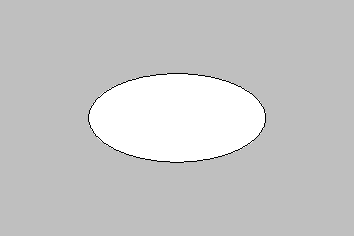
\includegraphics[scale=1.1]{fig/4-2.pdf}
\caption{电磁振荡的过程}
\end{figure}

电容器开始放电后,由于线圈的自感作用,电路里的电流不能立刻达到最大值,而是由零逐渐增大,放电过程中,线圈周围产生磁场,并且随着电流的增大而增强;电容器极板上的电荷逐渐减少,电容器里的电场逐渐减弱.这样,电路里的电场能逐渐转化为磁场能,到放电完了时,电流达到最大值,电容器极板上已经没有电荷,电场能全部转化为磁场能(图4.2乙).


电容器放电完了后,由于线圈的自感作用,电路里的电流并不立即减小为零,而是保持原来的方向继续流动,使电容器在反方向上重新充电.在反方向充电过程中,随着电流的减小,线圈周围的磁场逐渐减弱;电容器两极板带上相反的电荷,电容器里的电场随着极板上电荷的增多而增强.这样,电
路里的磁场能又逐渐转化为电场能,充电完了时,电流减小到零,电容器极板上的电荷达到最大值,磁场能全部转化为电场能(图4.2丙).

此后电容器再放电,再充电,这样不断地充电和放电,电路中就有了振荡电流,同时电场能和磁场能发生周期性的转化.这种现象叫做\textbf{电磁振荡}.

图4.2中的电磁振荡跟机械振动中的自由振动类似,叫做\textbf{自由振荡}.最初给电容器充电,相当于使单摆的摆锤偏离平衡位置,给摆锤一定的重力势能,电路中电场能和磁场能的相互转化,相当于单摆中重力势能和动能的相互转化.

\subsection{无阻尼振荡和阻尼振荡}

在自由振荡中,如果没有能量损失,振荡应该持续下去,振荡电流的振幅应该保持不变.这种振荡叫做\textbf{无阻尼振荡}(图4.3甲).可是,实际上在电磁振荡中总要有能量损失,一部分能量由于电路中有电阻而转化为热,还有一部分能量辐射到周围空间中去.这样,振荡电路
的能量逐渐损耗,振荡电流的振幅逐渐减小,直到最后停止下来.这种振荡叫做\textbf{阻尼振荡}(图4.3乙).
\begin{figure}[htp]\centering
\begin{tikzpicture}[>=latex, xscale=.6]
\draw[->](0,0)node[left]{$O$}--(13,0);
\draw[->](0,-1)--(0,1)node[right]{$i$};
\draw [very thick] plot[domain=0:3.1416*4, samples=1000] function{0.5*cos(4.5*x)} ;
\node at (6.5, -1.5){甲:无阻尼振荡};
\end{tikzpicture}

\begin{tikzpicture}[>=latex, xscale=.6]
    \draw[->](0,0)node[left]{$O$}--(13,0);
    \draw[->](0,-1)--(0,1)node[right]{$i$};
    \draw [very thick] plot[domain=0:3.1416*4, samples=1000] function{.5*exp(-0.2*x)*cos(4.5*x)} ;
    \node at (6.5, -1.5){乙:阻尼振荡};


\end{tikzpicture}
\caption{}
\end{figure}

实际工作中常常需要保持振幅不变的等幅振荡,这种等幅振荡要用\textbf{振荡器}来产生.振荡器靠晶体管(或电子管)周期地把电源的能量补充到振荡电路中,用来补偿振荡过程中的能量损耗,以维持等幅振荡.

\subsection*{练习一}
\begin{enumerate}
	\item 画一条按正弦规律变化的振荡电流的曲线,并在这条曲线上标出对应于图4.2甲、乙、丙、丁、戊各个时刻电流值的点.
	\item 在图4.2所示的电磁振荡中,何时电容器里的电场最强?何时线圈里的磁场最强?电场能和磁场能是怎样相互转化的?
	\item 把$LC$回路中产生的自由振荡跟单摆的简谐振动相对比,说明它们类似的地方.
\end{enumerate}


\section{电磁振荡的周期和频率}
电磁振荡完成一次周期性变化需要的时间叫做\textbf{周期},一秒钟内完成的周期性变化的次数叫做\textbf{频率}.

振荡电路里发生无阻尼自由振荡的周期和频率,叫做振荡电路的\textbf{固有周期}和\textbf{固有频率},简称振荡电路的周期和频率.

$LC$回路的周期和频率跟哪些因素有关呢?让我们改变
电容和电感的大小,重做图4.1的实验,可以看到:电容或电感增加时,周期变长,频率变低;电容或电感减小时,周期变短,频率变高.

上述现象可以这样来说明,加在电容器上的电压一定时,电容器的电容越大,它容纳的电荷就越多,放电和充电需要的时间就越长,因而周期就越长,频率就越低,线圈的电感越大,阻碍电流变化的作用就越强,放电和充电需要的时间就越长,因而周期就越长,频率就越低.

进一步的研究可以证明,周期$T$和频率$f$跟自感系数$L$和电容$C$的关系是:
\[T=2\pi\sqrt{LC},\qquad f=\frac{1}{2\pi\sqrt{LC}} \]
式中$T$、$f$、$L$、$C$的单位分别是秒、赫兹、亨利、法拉.

根据上述公式,选用适当的电容器和线圈,就可以使振荡电路的周期和频率符合我们的需要,要改变振荡电路的周期和频率,可以通过改变电容或电感的办法来实现.

\subsection*{练习二}
\begin{enumerate}
	\item 一个$LC$回路能够产生535千赫到1605千赫的电磁振荡,已知线圈的自感系数是300微亨,可变电容器的最大电容和最小电容各是多少?
	\item $LC$回路中的可变电容器的电容可从30皮法变到15皮法.要使这个回路的最低固有频率为1000千赫,线圈的自感系数应为多大?用这个线圈,回路的最高固有频率是多大?
	\item 如果把$LC$回路中电容为$C$的电容器用两个电容也为$C$的电容器串联起来代替,回路的固有周期怎样变化?如果不是串联而是并联,固有周期又怎样变化?
\end{enumerate}


\section{电磁场}

电磁振荡能够产生电磁波,为了说明这个问题,我们需要知道一些有关电磁场的知识,十九世纪六十年代,英国物理学家麦克斯韦(1831—1879)在总结前人研究电磁现象的基础上,建立了完整的电磁场理论,这个理论不仅全面地说明了当时已知的电磁现象,而且成功地预言了电磁波的存在.下面我们简要地介绍一下这个理论的要点.

麦克斯韦用场的观点分析了电磁感应现象,并作出结论:\textit{变化的磁场能够在周围的空间产生电场}.这是电磁场理论的第一个要点,如图4.4所示,在变化的磁场中放一个闭合
电路,电路中就产生感生电流,这是我们学过的电磁感应现象.我们知道,要产生电流,必须有使电荷做定向移动的电场
存在,现在闭合电路里有了电流,说明有电场存在;这个闭合电路中没有其他电源,这个电场只能认为是由于磁场的变化而产生的.麦克斯韦进一步认为,这个电场的产生,跟是否存在着闭合电路没有关系,只要磁场发生变化,在周围空间里就要产生电场.
\begin{figure}[htp]\centering
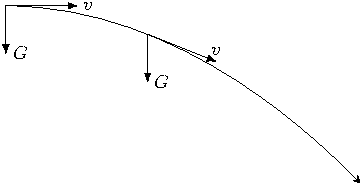
\includegraphics[scale=1.2]{fig/4-4.pdf}
\caption{变化的磁场产生电场(磁场增强时)}
\end{figure}

麦克斯韦还指出:变化的磁场所产生的电场,是由磁场的变化情况决定的,如果磁场的变化是均匀的,即在相等的时间内磁感应强度的变化相等,产生的电场就是稳定的,即电场强度不随时间而变化.如果磁场的变化是不均匀的,产生的电场就是变化的.

既然变化的磁场能够产生电场,相反地,变化的电场是否也能够产生磁场呢?麦克斯韦用场的观点分析了电磁现象,认为\textit{变化的电场能够在周围的空间产生磁场},这是电磁场理论的第二个要点,一个静止的电荷,它产生的是静电场,即空间各点的电场强度不随时间而变化,这个电荷一且运动起来,电场就发生变化,即空间各点的电场强度将随着时间而变化.另一方面,运动电荷要产生磁场.用场的观点来分析这个问题,就可以说:这个磁场是由变化的电场产生的,在电容器充放电时,两极板间的电场发生变化,这个变化的电场产生磁场(图4.5),而且这个磁场跟假定两极板间存在电流时所产生的磁场是一样的.
\begin{figure}[htp]\centering
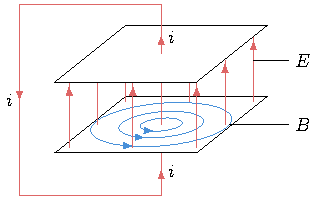
\includegraphics[scale=1.2]{fig/4-5.pdf}
\caption{变化的电场产生磁场}
\end{figure}


变化的电场所产生的磁场,是由电场的变化情况决定的.
如果电场的变化是均匀的,产生的磁场就是稳定的.如果电场的变化是不均匀的,产生的磁场就是变化的.

变化的磁场产生电场,变化的电场产生磁场,这是麦克斯韦理论的两大支柱.按照这个理论,变化的电场和磁场总是相互联系的,形成一个不可分离的统一的场,这就是电磁场.电场和磁场只是这个统一的电磁场的两种具体表现.

\section{电磁波}
\subsection{电磁波的产生}

从麦克斯韦的电磁场理论可以知道:如果在空间某处发生了不均匀变化的电场,就会在邻近的空间引起变化的磁场,这个变化的磁场又会在较远的空间引起新的变化的电场,接着又在更远的空间引起新的变化的磁场,这样,变化的电场和变化的磁场并不局限于空间某个区域,而要由近及远向周围空间传播开去,电磁场这样由近及远地传播就形成\textbf{电磁波}.
\begin{figure}[htp]\centering
\begin{tikzpicture}[>=latex, scale=1.1]
	\draw[pattern=north east lines](-.8,-.8) rectangle (.8,-.6);
	\draw[pattern=north east lines](-.8,.8) rectangle (.8,.6);
	\draw(0,.8)--(0,1.5);
	\draw(0,-.8)--(0,-1.5);
	\foreach \x in {0,3,-3}
	{
		\draw[thick](\x,0) ellipse [x radius=.9, y radius=.3];
	}
	\foreach \x in {1.5,-1.5}
	{
		\draw[dashed, thick](\x,0) circle (.8);
		\node at (\x,1){$E$};
	}
	\draw[dashed, thick](4.5,.8)node[above]{$E$} arc (90:270:.8);
	\draw[dashed, thick](-4.5,.8)node[above]{$E$}  arc (90:-90:.8);
	\foreach \x in {-.6,-.4,-.2,...,.4,.6}
	{
		\draw[dashed](\x,-.6)--(\x,.6);
	}
	
	\node at (3,.5){$B$};
	\node at (-3,.5){$B$};
	
	\draw[dashed](-.8,-.6)[bend left=30] to (-.8,.6);
	\draw[dashed](.8,-.6)[bend left=-30] to (.8,.6);
	
	
\end{tikzpicture}
\caption{电磁波传播过程的示意图}
\end{figure}

在图4.1所示的振荡电路中有振荡电流时,会产生周期性变化的电场和磁场,这种电场和磁场的变化是不均匀的,因而会激起电磁波向外传播(图4.6).电磁波的周期和频率等于激起电磁波的振荡电流的周期和频率,振荡电路中有振荡
电流时,电荷做快速振动,可见做快速振动的电荷会激起电磁波.

\subsection{电磁波的特点}
\begin{figure}[htp]\centering
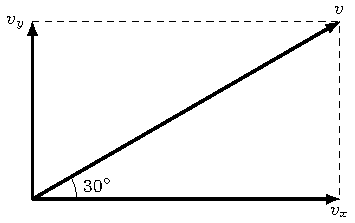
\includegraphics[scale=1.2]{fig/4-7.pdf}
\caption{沿$z$轴传播的电磁波在某一时刻的波的图象}
\end{figure}

图4.7表示作正弦变化的电场或磁场所
引起的电磁波在某一时刻的波的图象.波峰表示在该点的电场强度$E$或磁感应强度$B$在正方向具有最大值,波谷表示在该点的$E$或$B$在反方向具有最大值.两个相邻的波峰(或波谷)之间的距离等于电磁波的波长.在任一时刻,$E$和$B$沿电磁波的传播方向是作正弦变化的,在传播方向上的任一点,$E$和$B$都是随时间作正弦变化的,即$E$和$B$在振动.$E$的振动方向平行于$x$轴,$B$的振动方向平行于$y$轴,它们彼此垂直,而且都跟波的传播方向垂直,因此电磁波是横波.
\begin{figure}[htp]\centering
\begin{tikzpicture}[>=latex, xscale=.5]
\foreach \x in {0,2,4}
{
   \draw[->] (-.5, \x)--(20,\x)node [right]{$z$};
\draw [->](0,-.8+\x)--(0,1+\x)node [right]{$E$};
\node at (-.25,\x-.25){$O$};
}

\draw [very thick] plot[domain=0:4*3.1416, samples=1000] function{.7*sin(x)+4} ;
\draw [very thick] plot[domain=0:5*3.1416, samples=1000] function{-.7*sin(x)+2} ;
\draw [very thick] plot[domain=0:6*3.1416, samples=1000] function{.7*sin(x)} ;

\foreach \x in {1,2,3}
{
\draw[dashed] (2*3.1416*\x, -1)--(2*3.1416*\x, 5);
}

\draw[<->] (4*3.1416, 4.5) to node [fill=white]{$\lambda$} (6*3.1416, 4.5);

\node at (-4, 0){丙};\node at (-4, 4){甲};\node at (-4, 2){乙};
\node at (-2, 0){$t=T$};\node at (-2, 4){$t=0$};\node at (-2, 2){$t=\dfrac{1}{2}T$};

\draw[->] (3.1416/2, 0)--(3.1416/2, 0.7);
\draw[->] (3.1416/2, 2)--(3.1416/2, 2-0.7);
\draw[->] (3.1416/2, 4)--(3.1416/2, 4+0.7);

\draw[->] (3.1416*1.5, 0)--(3.1416*1.5, -0.7);
\draw[->] (3.1416*1.5, 2)--(3.1416*1.5, 2+0.7);
\draw[->] (3.1416*1.5, 4)--(3.1416*1.5, 4-0.7);

\draw[->] (3.1416/4, 0)--(3.1416/4, 0.7/1.414);
\draw[->] (3.1416/4, 2)--(3.1416/4, 2-0.7/1.414);
\draw[->] (3.1416/4, 4)--(3.1416/4, 4+0.7/1.414);

\draw[->] (3.1416*.75, 0)--(3.1416*.75, 0.7/1.414);
\draw[->] (3.1416*.75, 2)--(3.1416*.75, 2-0.7/1.414);
\draw[->] (3.1416*.75, 4)--(3.1416*.75, 4+0.7/1.414);

\draw[->] (3.1416*1.25, 0)--(3.1416*1.25, -0.7/1.414);
\draw[->] (3.1416*1.25, 2)--(3.1416*1.25, 2+0.7/1.414);
\draw[->] (3.1416*1.25, 4)--(3.1416*1.25, 4-0.7/1.414);

\draw[->] (3.1416*1.75, 0)--(3.1416*1.75, -0.7/1.414);
\draw[->] (3.1416*1.75, 2)--(3.1416*1.75, 2+0.7/1.414);
\draw[->] (3.1416*1.75, 4)--(3.1416*1.75, 4-0.7/1.414);

\end{tikzpicture}
\caption{电磁波以一定速度在空间传播(为简单起见只画出了$E$矢量)}
\end{figure}

电磁波在空间以一定的速度传播,图4.8表示经过一个周期$T$电磁波向前传播的情形.可以看出,经过一个周期$T$,电磁波传播的距离等于波长$\lambda$.因此,我们在高中一年级学过的波长、频率(或周期)和波速之间的关系,即$v=\lambda/T=\lambda f$,对电磁波也完全适用.

麦克斯韦从理论上预见:电磁波在真空中的传播速度等于光在真空中的传播速度,即电磁波在真空中的传播速度$c=3.00\x10^8\ms$,这个论断后来得到了实验证实.从理论上发现电磁波以光速传播,这是物理学史上最伟大的成就之一.后面我们学到光学时还要说明这一点.

从场的观点来看,必须把场看作能量的贮存场所,电场
贮存电能,磁场贮存磁能,电磁场贮存电磁能.因此,电磁波的发射过程,也就是辐射能量的过程.电磁波在空间传播,电磁能就随同着一起传播.

电磁波虽然可以由做快速振动的电荷所激起,但它可以脱离电荷而独立存在,设想一个振动的电荷突然停止运动,它的场就变成了静电场.原先它所激起的电磁波并不随同消失,而是在空间继续传播着.这时电磁波独立地存在着,我们可以象研究任何其他事物的变化过程一样来研究电磁波的变化过程.

电磁波有一点跟机械波大不相同,机械波要靠媒质来传播,电磁波可以在真空中传播,它的传播并不需要靠别的物质来做媒质;由于变化的电场和变化的磁场具有密不可分的联系,电磁波本身就能够传播.

电磁波可以脱离电荷而独立存在,并且不需要别的物质来做媒质就能够在空间传播,电磁波也具有能量.这样看来,电磁场跟由原子、分子组成的物质(通常叫做实物)一样,都是不依赖于我们感觉的客观存在,电磁场是物质的一种特殊形态.

现在让我们引用大科学家爱因斯坦的话作为本节的结束.他说:“在麦克斯韦的理论中,电场和磁场,或简单些说电磁场,是一种实在的东西”,“在一个现代物理学家看来,电磁场正和他所坐的椅子一样地实在”,“对目前来说,我们仍然需要认定场与实物都一起存在”.(引自爱因斯坦,英费尔德著:《物理学的进化》)

\section{赫兹实验}
麦克斯韦从理论上预见电磁波的存在,在这个预见以后,过了二十多年,在1888年,德国物理学家赫兹(1857—1894)第一次用实验证实了电磁波的存在.

\begin{figure}[htp]\centering
	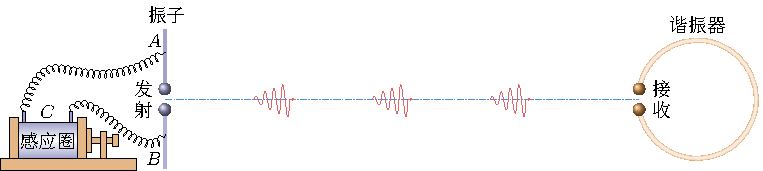
\includegraphics[scale=1]{fig/4-9.PDF}
	\caption{赫兹实验}
	\end{figure}

赫兹实验的原理如图4.9所示.左方是电磁波发射器,$A$和$B$是两根金属杆,它们相对的那端各带一个金属球,两球之间留有间隙,把两杆接到感应圈$C$的两极上.感应圈是一个特殊的变压装置,它可以把低电压变成高电压.当两金属
球之间的电压足够高时,空气被击穿,在两球间隙中发生火花放电,每跳一次火花,电荷在两球之间往复多次,形成高频的振荡电流.火花放电是间断性的,跳过一次火花之后,接着跳过第二次火花,这样,就间断性地发射出电磁波.

图4.9右方是电磁波接收器,它是一个金属圆环,也留有
一个间隙,在间隙处环的两端带有金属球,当电磁波传到接
收器时,电磁波的电场使环的两个金属球间产生电压,这个电压足够高时,在两球间隙中就会发生火花放电.

赫兹发现,在发射器的间隙有火花跳过时,接收器的间隙确有火花跳过,这样,赫兹用实验证实了电磁波的存在,赫兹还用实验测定了电磁波的波长和频率,得到了电磁波的传播速度,证实了这个速度等于光速.赫兹还用实验证明,电磁波跟所有波动现象一样,能产生反射、折射、干涉、衍射等现象,从而充分证实了麦克斯韦的电磁场理论.

今天,赫兹实验以及类似的实验很容易做成,我们在教室里就可以进行演示,在赫兹实验中电磁波传播的距离不过几米,而现在发射的电磁波可以传到几千千米的远处,麦克斯韦的理论成了无线电技术的基础.

\subsection*{练习三}
\begin{enumerate}
	\item 从地球向月球发射电磁波,经过多长时间才能在地球上接收到反射回来的电磁波?地球到月球的距离为$3.84\x10^5$千米.
	\item 我国第一颗人造地球卫星采用20.009兆赫和19.995兆赫的频率发送无线电信号,这两种频率的电磁波的波长各是多少?
	\item 有一台收音机,它接收的波长范围由560.7米到186.9米,它接收的频率范围是多少?
	\item 一个振荡电路辐射出的电磁波的波长是300米,这个振荡电路的周期是多大?
\end{enumerate}

\section{电磁波的发送(一)~~开放电路}
从赫兹成功地证实电磁波的存在,到现在不过一百年,电磁波在科学技术上已经得到广泛的应用.广播电台和电视台每天都在发射强大的电磁波,它带着能量和信号传到各地,我们打开收音机和电视机,就听到声音,看到图像(图4.10).这是怎样实现的呢?从这一节开始我们将学习有关这方面的一些基本知识.
\begin{figure}[htp]\centering
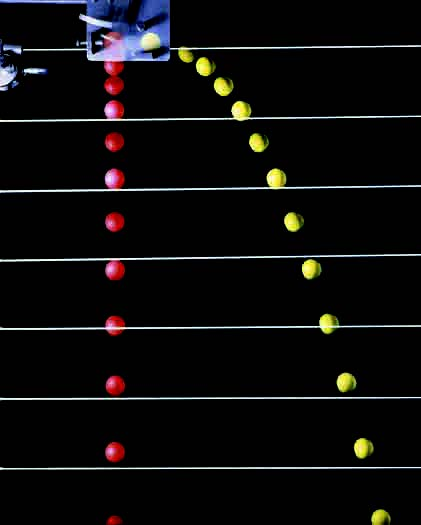
\includegraphics[scale=.45]{fig/4-10.png}
\caption{电磁波的发送和接收}
\end{figure}

\begin{figure}[htp]\centering
	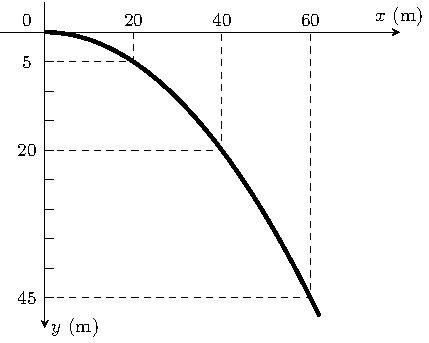
\includegraphics[scale=1.2]{fig/4-11.pdf}
	\caption{由闭合电路变成开放电路}
	\end{figure}

要利用电磁波,必须有效地向外发射电磁波.但是,由普通的电容器和线圈组成的振荡电路(图4.11甲),向外辐射能量的本领是很差的.这种振荡电路通常叫做闭合电路,电场和磁场几乎完全集中在电容器和线圈内,电场能和磁场能主要是在电路内互相转化,辐射出去的能量极少,实际上不能用来发射电磁波,为了有效地发射电磁波,必须尽可能使电场和磁场分散开.如果把电路改成图4.11乙那样,辐射能量的本领会好些;如果改成图4.11丙那样,辐射能量的本领就更好了,图4.11丙所示的电路叫做开放电路.

实际应用的开放电路,线圈下部用导线接地,这条导线叫做地线;线圈上部接到比较高的导线上,这条导线叫做天线.天线和地线形成了一个敞开的电容器.

研究表明,振荡电路辐射能量的本领跟振荡频率有关.电磁振荡的频率越高,向外辐射能量的本领就越大.因此,在无线电技术中使用的振荡电流频率都很高,在几百千赫以上.由
频率公式$f=\dfrac{1}{2\pi\sqrt{LC}}$知道,要提高振荡频率,必须降低振荡
电路的电感和电容.上面讲的具有天线和地线的开放电路,不但形式开敞,同时它的电感和电容都很小,有很高的固有频率,这对于发射电磁波是很有利的.
\begin{figure}[htp]\centering
\begin{circuitikz}[>=latex]
\draw (0,3)-- (2,3) to [american inductor] (2,0)-- (0,0)  ;
\draw (2.5, -.5) node [ground]{地线} to(2.5,0) to [american inductor] (2.5,3)to (2.5,3.5)node[bareantenna]{天线} ;
\draw (-.2, .5) rectangle (.2,2.5);
\draw (0,0)--(0,.5);
\draw (0,2.5)--(0,3);
\node [rotate=90]at (-.5,1.5){振荡器};
\node at (1.75,1.5){$L_2$};
\node at (2.75,1.5){$L_1$};
\end{circuitikz}
\caption{感应耦合}
\end{figure}

使开放电路里产生振荡电流,通常用如图4.12所示的感
应耦合的办法,使开放电路的线圈$L_1$跟振荡器电路中的线圈$L_2$接近.这样,振荡器电路里有振荡电流时,由于$L_2$和$L_1$的互感作用,在开放电路里就产生了同样频率的振荡电流,从而发射出电磁波.

无线电技术中使用的电磁波通常叫做\textbf{无线电波},无线电波的波长从几毫米到几十千米,例如中央人民广播电台发射一种频率为15.55兆赫的无线电波,波长为19.3米.通常根
据波长或频率把无线电波分成几个波段,如下表所示.

\begin{center}
\begin{tabular}{cp{.18\textwidth}p{.18\textwidth}cp{.25\textwidth}}
	\hline
	波段  &  波长  & 频率 & 传播方式 & 主要用途
\\
\hline
长波    &  30000—3000m  & 10—100KHz   &地波    & 超远程无线电通讯和导航\\
中波   & 3000—200m   & 100—1500KHz   & 地波和天波   & 无线电广播和电报通讯\\
中短波   & 200—50m   & 1500—6000KHz  & 地波和天波   & 无线电广播和电报通讯\\
短波 & 50—10m   & 6—30MHz & 天波   & 无线电广播和电报通讯\\
米波 & 10—1m   & 30—300MHz   & 近似直线传播   &  无线电广播、电视、导航\\
分米波 & 10—1dm   & 300—3000MHz   & 直线传播   &  电视、雷达、导航\\  
厘米波& 10—1cm   &  3000—30000MHz   & 直线传播   &  电视、雷达、导航\\ 
毫米波 & 10—1mm 
  & 30000—300000MHz   & 直线传播   &  电视、雷达、导航\\
\hline
\end{tabular}

\end{center}


\section{电磁波的发送(二)~~调制}
发射电磁波是为了用它来传递信号,无线电报传递的是
电码符号,无线电广播传递的是声音,无线电视传递的不仅有声音还有图像,怎样利用电磁波把电码、声音、图像等信号发射出去呢?

无线电技术中发射信号,先把要传递的信号转变为电信号,这种电信号频率比较低,不能直接用来发射电磁波,如果把这种电信号“加”到高频等幅振荡电流上,那么,载有信号的高频振荡电流产生的电磁波就载着要传递的信号一起发射出去,把要传递的电信号“加”到高频等幅振荡电流上叫做\textbf{调制}.进行调制的装置叫做\textbf{调制器}.要传递的电信号叫做调制信号.

常用的调制方法有\textbf{调幅}和\textbf{调频},调幅是使高频振荡电流的振幅随着调制信号而改变,调频是使高频振荡电流的频率随着调制信号而改变.

\begin{figure}[htp]
\centering
\begin{minipage}[t]{0.48\textwidth}
\centering
\begin{circuitikz}[>=latex]
\draw (0,3)to  (2,3) to [american inductor] (2,0) to [mic] (0,0)  ;
\node [waves,rotate=90] at(1,-1.75) {};
\draw (2.5, -.5) node [ground]{} to(2.5,0) to [american inductor] (2.5,3)to (2.5,3.5)node[bareantenna]{} ;
\draw (-.2, .5) rectangle (.2,2.5);
\draw (0,0)--(0,.5);
\draw (0,2.5)--(0,3);
\node [rotate=90]at (-.5,1.5){振荡器};
\node at (1.75,1.5){$L_2$};
\node at (2.75,1.5){$L_1$};

\end{circuitikz}
\caption{调制}
\end{minipage}
\begin{minipage}[t]{0.48\textwidth}
\centering
	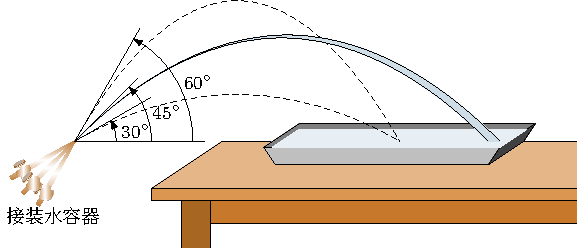
\includegraphics[scale=1.2]{fig/4-14.pdf}
	
	甲:高频等幅振荡电流的波形;乙:声音信号的波形;丙:经过调幅的高频振荡电流的波形
	\caption{调幅的作用}
\end{minipage}
\end{figure}


图4.13是调幅装置的示意图,接在振荡器和线圈$L_2$之间的话筒就是一个最简单的调制器.由声源发出的声音振动使话筒里的碳粒发生时松时紧的变化,它的电阻也发生时大时小的变化,所以,虽然振荡器产生的是高频等幅振荡电流
(图4.14乙),但在线圈$L_2$中通过的却是振幅随声音而改变的高频调幅电流(图4.14丙).由于$L_2$和$L_1$的互感作用,通过开放电路中的也是这种高频调幅电流,于是从开放电路就发射出振幅随声音面改变的电磁波.这种电磁波叫做\textbf{调幅波}.

根据这节和前节所讲的,我们看到,在电磁波的发送中必须有振荡器、调制器、天线和地线.振荡器产生高频等幅振荡电流,经过调制器后,成为被调制的高频振荡电流,于是开放电路就发射出带有调制信号的电磁波.为了使电磁波能传得
很远,还需要用放大器把被调制的高频振荡电流加以放大,以增强开放电路发射电磁波的功率,整个发送装置的方框图如图4.15所示.
\begin{figure}[htp]\centering
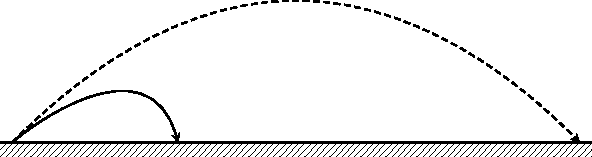
\includegraphics[scale=.45]{fig/4-15.png}
\caption{电磁波发送的方框图}
\end{figure}

\section{电磁波的接收(一)~~电谐振}
电磁波在空间传播时,如果遇到导体,就把自己的一部分能量传给导体,使导体中产生感生电流.感生电流的频率跟激起它的电磁波的频率相同.因此,利用放在电磁波传播空间中的导体,就可以接收到电磁波.无线电技术中,用天线和地线组成的接收电路来接收电磁波.

世界上有许许多多的无线电台,它们发出的电磁波的频
率各不相同,我们首先要从这些电台发出的电磁波中把我们要接收的选出来,通常这叫做选台.不进行选台,例如在收音机中,如果同时把各个广播电台发出的电磁波都接收下来,
并且把它们都转变成声音,那只能是一片嘈杂声,什么也听不清楚.怎样才能从许多电台中选出我们需要的那个电台呢?这就要设法使它发出的电磁波在接收电路里激起的感生电流最强,而其他电台发出的电磁波激起的感生电流都非常弱.

在无线电技术里是利用电谐振现象来实现这一点的,电谐振相当于机械振动中的共振,下面说明这种现象.

用莱顿瓶\footnote{莱顿瓶是由玻璃圆筒和贴在玻璃筒内外面上的锡箔构成的.它是一个电容器,两层锡箔是电容器的两极,它们之间的玻璃是电介质.内层的锡箔跟伸到瓶口外的带有金属球的金属棒相连接.}和带有间隙$AB$的矩形线圈组成第一个电路
(图4.16甲),用同样的莱顿瓶和带有氖管的一边可移动的矩形线圈组成第二个电路(图4.16乙).莱顿瓶具有电容,矩形线圈具有电感,所以这两个电路都是振荡电路.
\begin{figure}[htp]\centering
	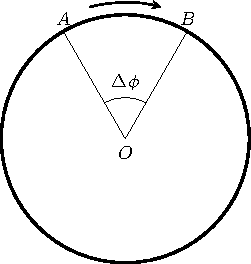
\includegraphics[scale=.45]{fig/4-16.png}
	\caption{电谐振}
	\end{figure}

给第一个电路中的莱顿瓶带电,当$AB$间的电压达到一定程度时,$AB$间就发生火花放电,这时移动第二个电路中矩形线圈的可移动的一边,可以看到:两个矩形线圈的大小相差不
多时,氖管开始发光;两个线圈的大小完全相同时,氖管最亮.

第一个电路实际上是电磁波发射器,跟赫兹实验中的发射器一样,发生火花放电时向外发射电磁波,电磁波的频率等于第一个电路的固有频率.第二个电路实际上是电磁波接收器,当它接收到第一个电路发射的电磁波时,就在电路中激起振荡电流,上面的实验说明激起的振荡电流的强弱跟接收电路的固有频率有关系.当两个线圈的大小完全相同时,它们的自感是相同的;而两个莱顿瓶是一样的,它们的电容也相同.因此两个电路的固有频率相同,这就是说,当接收电路的固有频率跟接收到的电磁波的频率相同时,激起的振荡电流最强,这就是电谐振现象.

使接收电路产生电谐振的过程叫做\textbf{调谐},能够调谐的接收电路叫做调谐电路.
\begin{figure}[htp]\centering
\begin{circuitikz}[>=latex]
    \draw (0,0) to [vC] (0,3) --(2,3)to  [american inductor](2,0)--(0,0);
    \draw (1, 3) to(1,4) node [bareantenna]{} ;
    \draw (1, 0) to(1,-.5) node [ground]{} ;
    \draw (1, 0) [fill=black] circle (1.5pt);
    \draw (1, 3) [fill=black] circle (1.5pt);
\end{circuitikz}
	\caption{调谐电路}
	\end{figure}

图4.17是收音机的调谐电路.调节可变电容器的电容来改变调谐电路的频率,使它跟我们要接收的电台发出的电磁波的频率相同,由于电谐振现象,只有这个频率的电磁波才在调谐电路里激起较强的感生电流,这样,我们就可以选出需要的电台.

\section{电磁波的接收(二)~~检波}
由无线电台发射出的是经过调制的载有信号的电磁波,
在调谐电路中因电谐振而产生的也是经过调制的高频振荡电流.这种电流通过收音机的耳机或扬声器,并不能使它们振动而发声.为什么呢?假定某一个半周期电流的作用是使振动片向某个方向运动,下一个半周期电流就以几乎同样大的作用使振动片向反方向运动,高频电流的周期非常短,半周期更短,而振动片的惯性相当大,所以在振动片还没有来得及在电流的作用下向某个方向运动的时候,就立刻有一个几乎同样大的作用要使它向反方向运动,结果振动片实际上不发生振动,因此,在电磁波的接收中还必须设法从经过调制的高频振荡电流中取出发射时加上去的调制信号.

从经过调制的高频振荡电流中取出调制信号的过程,叫做\textbf{检波}.检波是调制的逆过程,也叫做解调.由于调制的方法不同,检波的方法也不同,下面介绍收音机中对调幅波的检波.
\begin{figure}[htp]\centering
\begin{circuitikz}[>=latex]
\draw (0,0) to [vC] (0,3)--(1.8,3) to [american inductor] (1.8,0)--(0,0);
\draw (.9, 0) to(.9,-.5) node [ground]{} ;
\node at (-.75,1.5){$C_1$};\node at (1.6,1.5){$L_1$}; \node at (2.8,1.5){$L_2$};
\ctikzset{diodes/scale=0.6}  \draw (2.6,0) to  [american inductor] (2.6,3) to [full diode=$D$](5,3)--(6,3)to [mic=耳机](6,0) -- (0,0) ;
\draw (5,0)to [C=$C_2$, *-*] (5,3);
\draw (.9, 3) to(.9,3.9) node [bareantenna]{} ;

\draw[dashed](2.2, 0)--(2.2,3.5);\draw[dashed](3.2, -.5)--(3.2,3.5);
\draw (2.6,0) [fill=black] circle (1.5pt);
\draw (1.8,0) [fill=black] circle (1.5pt);
\draw (.9, 0) [fill=black] circle (1.5pt);
\draw (.9, 3) [fill=black] circle (1.5pt);
\end{circuitikz}
\caption{}
\end{figure}

图4.18虚线的右边是晶体二极管的检波电路,是利用晶体二极管的单向导电性来进行检波的.$L_1C_1$调谐电路中产生的是经过调幅的高频振荡电流(图4.19甲).$L_1$和$L_2$绕在同一磁棒上,由于互感作用,在$L_2$上产生的是高频交变电压.由于晶体二极管$D$有单向导电性,通过它的是单向脉动电流
(图4.19乙).这个单向脉动电流既含有高频成分,又含有音频成分.由于电容器有通高频阻低频的作用,高频成分基本上从电容器$C_2$通过,剩下的音频电流(图4.19丙)通过耳机,
使耳机的振动片随着信号而振动发声.
\begin{figure}[htp]\centering
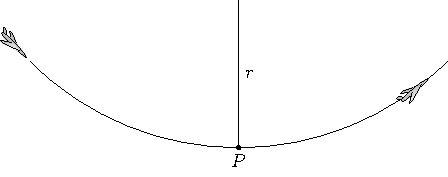
\includegraphics[scale=.45]{fig/4-19.png}
\caption{检波的作用}
甲:高频调幅电流的波形,乙:检波后的脉动电流的波形,丙:通过耳机的音频电流的波形.
\end{figure}

图4.18实际上就是一个晶体二极管收音机的电路图.这种收音机声音很小,只能用耳机收听本地电台.为了提高收音机的接收性能,需要用放大器把微弱的信号放大,图4.20是加有放大器的收音机方框图.由天线和调谐电路接收到的高频调幅电流,先通过放大器进行高频放大,然后进行检波和
低频放大,放大后的音频电流通过耳机或扬声器,使它们发出声音,在学生实验中,我们将熟悉这种收音机的电路图,并且要根电路图进行收音机的安装和调试.
\begin{figure}[htp]\centering
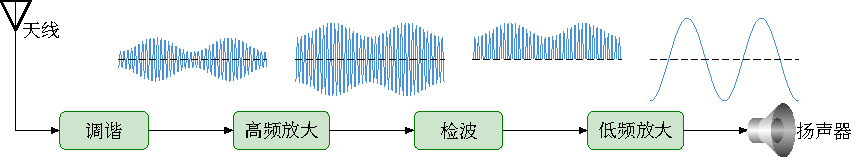
\includegraphics[scale=.45]{fig/4-20.png}
\caption{收音机的方框图}
\end{figure}


\subsection*{练习四}
\begin{enumerate}
	\item 有一台收音机,把它的调谐电路中的可变电容器的动片从完全旋入到完全旋出,仍然接收不到某一较高频率电
	台的信号,要想接收到该电台的信号,应该增加谐振线圈的匝
	数,还是减小谐振线圈的匝数?为什么?
	\item 收音机由收听某一较高频率的电台改为收听某一较低频率的电台,调谐电路中可变电容器的动片应该旋进一些还是旋出一些?为什么?
	\item 某收音机调谐电路的可变电容器的动片完全旋入时,电容是390皮法,这时能接收到520千赫的无线电波.动片完全旋出,电容变为39皮法,这时能接收到的无线电波的频率是多大?在这两种情形下,接收到的电磁波的波长分别是多长?
\end{enumerate}

\section{传真~~电视~~雷达}
这一节我们介绍无线电波的现代应用——传真、电视和雷达的原理.

\subsection{传真}

无线电传真是利用无线电波传送图表、书信、照片等图像的一种方法,报纸印的许多照片都是传真照片.

跟无线电广播不同,在无线电传真中要把图像反射出的光转换为电信号.光电管的制成解决了这个问题.利用光电管可以使电流随着光的强弱而改变,光电管是传真装置中的主要元件,光电管的原理将在本书第七章介绍.
\begin{figure}[htp]\centering
	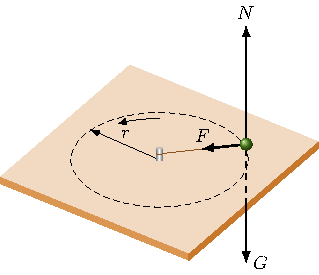
\includegraphics[scale=.45]{fig/4-21.png}
	\caption{无线电传真示意图}
	\end{figure}

在发射端,把图片贴在图4.21左方的转动筒上,转动筒在光电管近旁,一边转动,一边沿轴向移动.这样,图片各部分反射出的强弱不同的光,按照一定顺序照射到光电管上,在光电管电路中就出现了强弱变化的信号电流.用光电管电路作调制器,把信号电流调制到高频等幅振荡电流上,经过发射机
就发射出带有传真信号的无线电波.

在接收端,接收机收到带有传真信号的无线电波后,经过放大、检波,把传真信号取出并送给辉光管,辉光管是一种充气管,它发出的光的强弱随着通过的电流的强弱而变化.这样,辉光管所发的光的强弱变化,跟发射端图片各部分的反射光的强弱变化相同.辉光管发的光会聚到卷在转动筒上的感
光纸上,接收端用的转动筒跟发射端的相同,移动和转动的情况也完全一致,感光纸依次曝光,再经过显影、定影,就得到跟原来一样的图片.

\subsection{电视}

传真传递的是静止的图像,电视传递的是活动的景像,电视的活动景像是怎样形成的呢?
\begin{figure}[htp]\centering
	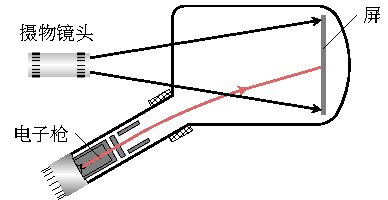
\includegraphics[scale=.45]{fig/4-22.png}
	\caption{摄像管}
	\end{figure}

在电视的发射端,摄取景物并将景物反射的光转换为电信号,是由摄像管(图4.22)来完成的,摄像时,摄像镜头将
被摄物体的像成在摄像管中的屏上.电子枪发出的电子束按一定规律偏转,对屏上的图像进行扫描,扫描的路线如图4.23所示,从$a$开始,逐行进行,直到$b$.这样,把一幅图像各个部分的明暗情况逐点变成强弱不同的信号电流,经过发射机就发射出带有图像信号的无线电波.
\begin{figure}[htp]
	\centering
	\begin{minipage}[t]{0.48\textwidth}
	\centering
	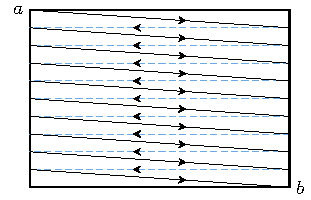
\includegraphics[scale=1.2]{fig/4-23.pdf}
	\caption{扫描}
	\end{minipage}
	\begin{minipage}[t]{0.48\textwidth}
	\centering
	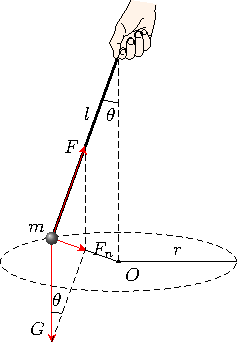
\includegraphics[scale=1.2]{fig/4-24.pdf}
	\caption{显像管}
	\end{minipage}
	\end{figure}
	
在电视接收端,把电信号转换成景物的像,是由显像管(图4.24)来完成的.电视机接收到带有图像信号的无线电波后,经过放
大、检波,把图像信号送到显像管,显像管里也有一个电子枪,它发射电子束的强弱受图像信号的控制,并且按照跟摄像管的电子枪同样的步调和方式扫描,这样,当电子束射到显像管底部的荧光屏上时,在屏上就出现跟摄像管屏上相同的图像.

摄像机在1秒钟内要传送25张画面,电视机也以相同的速率在荧光屏上显现这些画面.由于画面更换迅速和视觉暂留,我们便看到了活动的影像.

电视机接收到的无线电波,除了带有图像信号,还带有伴音信号,伴音信号经检波取出后,送入扬声器,扬声器就伴随着活动景像发出声音来.

从二十世纪二十年代开始试验电视广播以来,电视技术有了很大的发展,已由黑白电视发展到彩色电视.电视技术目前仍在迅速发展中.

电视的应用日益扩大,除了电视广播,有线电视(又叫闭路电视)也得到了广泛应用.例如,在自动化企业的控制中心,可以利用电视来监视各条生产线的工作情况.一些不便直接观察的地方,如有毒气或强烈放射性的地方,可以用电视作间接的观察.现在,电视技术已经应用到工业、交通、文化教育、国防和科学研究等各个方面.

\subsection{雷达}

雷达是利用无线电波来测定物体位置的无线电设备.

电磁波遇到障碍物要发生反射,雷达就是利用电磁波的反射来工作的.波长越短的电磁波,传播的直线性越好,反射性能越强,因此雷达用的是微波波段的无线电波.

雷达有一个特制的可以转动的天线(图4.25),它能向一定的方向发射不连续的无线电波,每次发射的时间约为百万分之一秒,两次发射的时间间隔大约是发射时间的一百倍.发射出去的无线电波遇到障碍物时,可以在这个时间间隔内反射回来为天线接收.
\begin{figure}[htp]\centering
	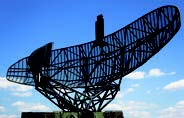
\includegraphics[scale=1.2]{fig/4-25.jpg}
	\caption{雷达天线}
	\end{figure}

已知无线电波的传播速度$c$,测出从发射无线电波到接收到反射回来的无线电波的时间$t$,就可以根据公式$2s=ct$来确定障碍物的距离,再根据发射无线电波的方向和仰角,便可以确定障碍物的位置.

实际上,障碍物的距离等情况是由雷达的指示器直接显示出来的,当雷达向目标发射无线电波时,在指示器的荧光屏上呈现出一个尖形波;在收到反射回来的无线电波时,在荧光屏上呈现出第二个尖形波(图4.26).根据两个波的距离,可直接从荧光屏上的刻度读出障碍物的距离.
\begin{figure}[htp]\centering
	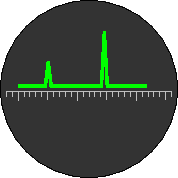
\includegraphics[scale=.45]{fig/4-26.png}
	\caption{}
	\end{figure}

利用雷达可以探测飞机、舰艇、导弹以及其他军事目标.除了军事用途外,雷达在交通运输上可以用来为飞机、船只导航,在天文学上可以用来研究星体,在气象上可以用来探测
台风、雷雨、乌云.

\section{电磁波的传播}
不同波长的电磁波有着不同的传播特性,这里只介绍无线电波的传播.无线电波的传播方式大致有三种:地波、天波和直线传播(图4.27).
\begin{figure}[htp]\centering
	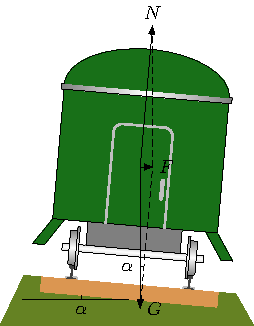
\includegraphics[scale=.45]{fig/4-27.png}
	\caption{}
	\end{figure}

\subsection{地波}

沿地球表面空间传播的无线电波叫做地波.

地面上有高低不平的山坡和房屋等障碍物,无线电波要绕过这些障碍物;才能被各处的接收机收到.波的重要特性之一是衍射,当波长大于或相当于障碍物的尺寸时,波可以绕到障碍物的后面,地面上的障碍物一般不太大,长波能很好地绕过它们.中波和中短波也能较好地绕过它们,短波和微波的波长过短,绕过障碍物的本领很差.

地球是导体,地波沿地面传播时地球表面会因电磁感应
而激起感生电流,这就要损失能量,这种能量损失随频率的增高而增大.因此,从能量损失的角度来看,这种传播方式对长波、中波和中短波比较适宜,对短波和微波则不适宜.

地波在传播过程中要不断损失能量,因此中波和中短波的传播距离不太大,一般在儿百千米范围内.收音机在这一波段一般只能收听到本地或附近省市的电台,就是这个缘故.虽然长波的传播距离可以远得多,但发射长波的设备庞大,造
价高,因此无线电广播一般不用长波,由于地波传播稳定可靠,近年来在超远程无线电通讯和导航技术等方面,发射长波的技术已有很大发展.

\subsection{天波}

依靠电离层的反射来传播的无线电波叫做天波.什么是电离层呢?在地球表面的大气层中,在大约50千米到几百千米的范围内,一部分中性气体分子由于受到太阳光的照射而发生电离,分解为带正电的离子和自由电子,这层大气就叫做电离层.

电离层对于不同波长的电磁波表现出不同的特性,对于波长短于10米的微波,电离层能让它穿过,飞向宇宙.对于波长超过3000米的长波,电离层基本上把它吸收掉.对于中波、中短波和短波,波长越短,电离层对它吸收得越少而反射得越多.因此,短波最适宜以天波的形式传播,可以传到几千千米以外的远处.

电离层是不稳定的,白天电离程度高,夜晚电离程度低.夜晚电离程度低,电离层对中波和中短波的吸收减弱,这时中波和中短波也可以用天波的形式传播.收音机在夜晚能够收听到许多远地的中波或中短波电台,就是这个缘故.由于电离层不稳定,电离程度和高度经常变化,无线电波到达接收机时强弱也随着时刻变化,因此在用一般收音机收听短波广播时,声音常是忽大忽小,高级收音机里,增设特殊的线路自动控制音量,来解决这个问题.

\subsection{直线传播}

微波又叫超短波,它既不能以地波的形式传播,又不能依靠电离层的反射以天波的形式传播.微波的传播形式跟光相似,是沿直线传播的.这种沿直线传播的无线电波叫做空间波或视波.

地球表面是圆球形的,沿直线传播的微波能够传播的距离不大,一般为几十千米.这种传播方式受大气的干扰小,能量耗损小,接收到的信号较强而且比较稳定,电视、雷达采用的都是微波.

远距离传送微波,需要设立中继站,由某地发射出的微波被中继站接收,放大后再传向下一站,这样一站传一站,把微波传向远方,同步通讯卫星可以用来作微波中继站.同步通讯卫星相对于地面静止在赤道上空36000千米的高处,只要有三颗这样的卫星,就可以把微波信号传遍全世界.

\section{电子技术一瞥}
前面讲过的无线电广播、电视、传真等通常叫做无线电技术,在无线电技术中,要利用各种电子器件如电子管、晶体管、摄像管、显像管、光电管等,也要利用无线电波在空间的传
播.电子技术是在无线电技术的基础上发展起来的,现在它已经大大超出了无线电技术的范围,成为一门领域十分广泛
的现代科学技术.可以说,凡是要用到各种电子器件的技术,不论是否利用电磁波在空间的传播,都属于电子技术的范围.示波器,收音机和电视机是电子技术的成果,电子显微镜和电子计算机也是电子技术的成果.

电子技术广泛地应用于工业、农业、国防等部门中,是现代化生产和科学研究的重要手段.电子技术在通讯方面的应用很广,除了广播和电视而外,还有无线电报、无线电话、无线电导航等,空间科学离不开电子技术.没有精确的电子测量和电子控制,卫星就不能上天.在工业上利用电子技术进行自动控制、自动调节、自动监视和保护等.各种程序控制机床是利用电子技术来自动控制的.自动调节可以把温度、压力、速度或液面高度准确地调节在一定数值.利用电子技术可以
自动监视机器的运转,有危险时能发出警报或采取保护措施.利用电子技术还能够实行遥控(远距离操纵),例如在一个地点可以同时控制远处的几座水电站的运行,利用电子技术可以作各种精密测量,例如用电子测微计能测出$10^{-8}$厘米的距离,利用电子技术还可以研究天文学、气象学、医学等.

电子计算机是二十世纪的重大发明,是电子技术的一项卓越成就.从电子计算机出现以来,已经经历了“四代”的变化.随着电子器件的微型化,即由电子管、晶体管到集成电路(在一小片半导体上制造出晶体管、电容、电阻等元件,并连接起来形成电路)、大规模集成电路(一般有几千个到几万个晶体管),并向着超大规模集成电路发展,七十年代以后出现了第四代电子计算机,不但有大中型电子计算机,应用于科学技术领域,而且出现了微型电子计算机(微电脑),微电脑的体积
小,耗能少,便宜可靠,便于推广使用,它在气象、水电、医疗、商业、军工、教育、财经、铁路、交通、邮电等领域取得广泛的应
用.微电脑的广泛应用和推广,将使整个生产结构和社会生活发生巨大变化.

电子技术的发展是世界范围的新技术革命的重要组成部分,以电子计算机为代表的电子技术水准已成为衡量一个国家现代化水平的重要标志.

我国的电子技术现在已经有了相当的发展.
在通讯方面,我国的广播和电视事业发展很快.广播已基本普及.到1983年底,全国拥有广播电台122座,发射的总功率是解放初期的250倍.全国拥有电视台52座,省以下的电视专业微波线路14156千米,电视覆盖地区的人口约占总人口的60\%.我国已经成功地发射了通信广播卫星,成为世界上少数几个能独立发射这种卫星的国家之一,这标志着我国卫星通信技术已接近世界先进水平.

我国于1958年就研制成功了第一台电子管元件计算机.此后陆续又研制出一批大、中、小型集成电路计算机,近年来,我国在集成电路的研制和生产、计算机的推广和应用等方面都取得了很大成绩.1983年我国成功地研制成每秒运算一亿次的“银河”巨型机.1984年我国在研制超大规模集成电路上取得了新的突破,我国的微电脑已批量定型生产.

我国的电子技术,目前虽然同国际先进水平还有差距,但
不久的将来一定会进入国际先进水平的行列,同学们在发展我国电子技术方面将会作出贡献.

\section*{复习题}
\begin{enumerate}
	\item 简述$LC$回路产生电磁报荡的过程.
	\item $LC$回路的周期和频率跟哪些因素有关?写出周期和频率的公式.
	\item 麦克斯韦电磁场理论的两个要点是什么?
	\item 电磁波是怎样产生的?为什么说电磁场是物质的一种特殊形态?
	\item 简述证实电磁波存在的赫兹实验.
	\item 发射电磁波为什么要用开放电路?又为什么要用高频振荡电流?
	\item 什么叫调制?什么叫调幅?设用音频电信号来调幅,画出调幅前后高频振荡电流的波形.
	\item 简述电谐振现象,什么叫调谐?在收音机电路里是怎样实现调谐的?
	\item 什么叫检波?晶体二极管的检波电路是怎样的?画出检波前后高频振荡电流的波形.
	\item 无线电波主要有几种传播方式?不同波段的无线电波各以什么方式传播?
\end{enumerate}

\section*{习题}
\begin{enumerate}
	\item 要使$LC$回路的固有频率增大,应该采用下述哪种方法?
	\begin{enumerate}
		\item 增大电容器两极板间的距离;
		\item 增大电容器两极板的正对面积;
		\item 在线圈中插入铁心;
		\item 减小线圈的匝数.
	\end{enumerate}
	\item 赫兹实验中的发射器为什么用图4.9那种形式,面不用该实验中接收器那种形式?赫兹实验中需要把接收器的两金属球调节到合适的距离,才有明显的接收效果,为什么?
	\item 回旋加速器中的磁感应强度为$B$,被加速的粒子的电量为$q$,质量为$m$.用$LC$振荡器作为高频电源,电感$L$和电容$C$的数值应该满足什么条件?
	\item 附近有电焊机进行电焊,或者有汽车通过,收音机和电视机会受到干扰,解释这个现象.
\end{enumerate}













